\newpage
\chapter{IOT Projects:}

The \ac{SPC} is a research lab, that is in constant development to show the latest innovations and bring them to use in industrial applications.
In the context of the master-thesis "Using FANUC R-2000iC/210F (6-axis robot) for improved efficiency in FRC parts formation" the topic of digital twinning and with that \ac{IOT} has become a major research point. 
In order to bring the \ac{FRC} production line to its full potential, several new projects could be defined. 
These projects improve comfort, energy-efficiency, ease of use and safety of the lab.
Each of these projects is designed to provide a flexible workload for 1-3 students with varying results depending on the students experience level and semester. In case 3 students sign up for a project, the diligence work is expected to be fulfilled. Each student is expected to pick their own range of tasks that they fulfil.
Following project ideas are proposed:\\
\bigskip
%
\section*{Room Temperature Control System}

	\begin{figure}[H]
	\centering
	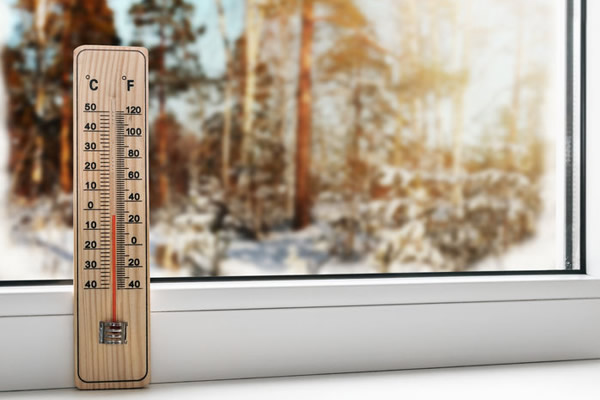
\includegraphics[
	width=0.5\linewidth,
	height=\paperheight,
	keepaspectratio,
	]{RoomTemp}
	\caption{Heating when noone needs it is waste! \cite{RoomTemp}}
	\label{fig: RoomTemp}
\end{figure}


The Lab of the \ac{SPC} has an old heating system controlled with electromechanical thermostats. 
Originally this system was designed to work with steam delivered by the \ac{IPKW}. 
Later this System was retrofitted with two gas heaters that have no feedback about the actual heating demand. This needs to be improved for comfort and energy-efficiency.\\
\\
Your assignment will be to replace the old and manual control with an open-source home automation system. That means choosing sensors, actuators, electronic components and clients as well as the type of home automation servers. 
A possible approach would be using thermocouples as sensors, transistors to switch the inputs of the heating system, using an ESP8266 for sensing and controlling with \ac{FHEM} as the underlying home automation server running on a raspberry pi.\\
diligence work: also include other room thermostats in the offices as well as lights\\
\\
Why are you the right one for this project? (Not all is required, but some should resonate with you)
\begin{itemize}
\item You are interested in automation systems
\item You like improving existing systems with electronics
\item You have experience with Arduino/ESP8266
\item You are not afraid to learn a new programming language to do some basic tasks
\item You like Linux
\item You like it warm and cozy in the morning :)
\end{itemize}
\bigskip
%
\section*{NFC based Machine Access}

	\begin{figure}[H]
	\centering
	
\includegraphics[
	width=0.5\linewidth,
	height=\paperheight,
	keepaspectratio,
	]{NFC}
	\caption{\ac{NFC} \cite{NFC}}
	\label{fig: NFC}
\end{figure}


The Lab of the \ac{SPC} has several heavy machines that move at high velocities, apply high pressures or create high temperatures. Because of these and other risks, a zoned safety system would make the lab a lot safer, as people would then stay in their assigned working zones while leaving work at other places unaffected. Also machine access needs to be restricted to the assigned student, while still leaving a traceable, temporarily restricted access to other users if necessary.\\
\\
Your assignment will be creating a \ac{NFC} card based zone and machine access. You can base this on an existing framework, or do it yourself. You will set up several \ac{NFC} readers with microcontrollers. These microcontrollers need to send a signal to a server that compares the access parameters delivered from the \ac{NFC}-card with a database that you set up. In case of a match, a signal is sent back to the Arduino, that switches a relay to open the gate. Additionally the Arduino should listen to other inputs in case a product cycle needs to be finished or additional requirements need to be fulfilled. Also there should be a signal sent back, when someone checks out of a safety zone. Machine access should have a timeout. Make a nice frontend to manage access.\\
diligence work: Make the communication between server and client hard to hack\\
\\
Why are you the right one for this project? (Not all is required, but some should resonate with you)
\begin{itemize}
\item You are interested in safety/security systems
\item You like to integrate something new into an ongoing project
\item You have experience with programming
\item You like microcontrollers
\item You can make a \ac{GUI}
\item (For diligence work: You like crypto)
\end{itemize}
\bigskip
%
%\section{Visual tool management system}
%In the lab of the \ac{SPC} many students use different tools like hammer, screwdrivers, wrenches etc. These tools get used throughout the day but rarely find their way back to their designated places (I'm also guilty of this). After spending a long time in the lab, many tools loose their designated storage places. It would be handy to take a photo of a tool and receive information about where to store it. Additionally, through the database the catalogue of available tools could be searched. \\
%\\
%Your assignment will be the creation of a program that can take a photo of a tool, recognize it and give out a description of its storage place with a photo. You will create a computer vision tool, probably based on machine learning to recognize the wide palette of tools in the lab.\\
%diligence work: Make it an android app\\
%\\
%Why are you the right one for this project? (Not all is required, but some should resonate with you)
%\begin{itemize}
%\item You are interested in image recognition
%\item You like to come up with something new
%\item You have experience with programming, ideally in Python
%\item (Diligence work: You would like to make an app)
%\item You don't like hardware
%\item You hate looking for stuff ;-)
%\end{itemize}
%\bigskip
%%